% XeLaTeX document
\documentclass[12pt,a4paper]{article}

% Редактируем: конфигурация, личные настройки: имя, название предмета и пр. для титульной страницы и метаданных документа здесь
\newcommand{\university}{Санкт-Петербургский политехнический университет Петра Великого}
\newcommand{\faculty}{Институт прикладной математики и механики}
\newcommand{\department}{Кафедра «Прикладная математика»}
\newcommand{\city}{Санкт-Петербург}
\newcommand{\num}{ №6}
\newcommand{\docname}{Отчёт по лабораторной работе}
\newcommand{\subject}{Математическая статистика}
\newcommand{\tutorname}{Баженов А. Н.}
\newcommand{\studentname}{Бавыкина М. А.}
\newcommand{\group}{3630102/70401}

% Не редактируем: используемые пакеты
% настройка кодировки, шрифтов и русского языка
\usepackage{fontspec}
\usepackage{polyglossia}

% рабочие ссылки в документе
\usepackage{hyperref}

% графика
\usepackage{graphicx}
\usepackage{tikz}
% поворот страницы
\usepackage{pdflscape}

% качественные листинги кода
\usepackage{minted}
\usepackage{listings}
\usepackage{lstfiracode}

% отключение копирования номеров строк из листинга, работает не во всех просмотрщиках (в Adobe Reader работает)
\usepackage{accsupp}
\newcommand\emptyaccsupp[1]{\BeginAccSupp{ActualText={}}#1\EndAccSupp{}}
\let\theHFancyVerbLine\theFancyVerbLine
\def\theFancyVerbLine{\rmfamily\tiny\emptyaccsupp{\arabic{FancyVerbLine}}}

% библиография
\bibliographystyle{templates/gost-numeric.bbx}
\usepackage{csquotes}
\usepackage[parentracker=true,backend=biber,hyperref=false,bibencoding=utf8,style=numeric-comp,language=english,autolang=other,citestyle=gost-numeric,defernumbers=true,bibstyle=gost-numeric,sorting=ntvy,]{biblatex}

% установка полей
\usepackage{geometry}

% нумерация картинок по секциям
\usepackage{chngcntr} 
\usepackage{subfigure}

% дополнительные команды для таблиц
\usepackage{booktabs}

% для заголовков
\usepackage{caption} 
\usepackage{titlesec}
\usepackage[dotinlabels]{titletoc}

% разное для математики
\usepackage{amsmath, amsfonts, amssymb, amsthm, mathtools}

% водяной знак на документе, см. main.tex
\usepackage[printwatermark]{xwatermark} 


% Не редактируем: параметры используемых пакетов и не только
% настройки polyglossia
\setdefaultlanguage{russian}
\setotherlanguage{english}

% локализация
\addto\captionsrussian{
  \renewcommand{\figurename}{Рисунок}%
  \renewcommand{\partname}{Глава}
  \renewcommand{\contentsname}{\centerline{Содержание}}
  \renewcommand{\listingscaption}{Листинг}
}

% основной шрифт документа
\setmainfont{CMU Serif}

% перечень использованных источников
\addbibresource{refs.bib}

% настройка полей
\geometry{top=2cm}
\geometry{bottom=2cm}
\geometry{left=2cm}
\geometry{right=2cm}
\geometry{bindingoffset=0cm}


% настройка ссылок и метаданных документа
\hypersetup{unicode=true,colorlinks=true,linkcolor=black,citecolor=green,filecolor=magenta,urlcolor=cyan,		       
    pdftitle={\docname},   	    
    pdfauthor={\studentname},      
    pdfsubject={\subject},      		        
    pdfcreator={\studentname}, 	       
    pdfproducer={Overleaf}, 		     
    pdfkeywords={\subject}
    }


% настройка подсветки кода и окружения для листингов
\usemintedstyle{colorful}
\newenvironment{code}{\captionsetup{type=listing}}{}

% шрифт для листингов с лигатурами
\setmonofont{FiraCode-Regular.otf}[
    Path = templates/,
    Contextuals=Alternate
]

% оформления подписи рисунка
\captionsetup[figure]{labelsep = period}

% подпись таблицы
%\DeclareCaptionFormat{hfillstart}{\hfill#1#2#3\par}
%\captionsetup[table]{format=hfillstart,labelsep=newline,justification=centering,skip=-10pt,textfont=bf}

% путь к каталогу с рисунками
\graphicspath{{fig/}}

% Внесение titlepage в учёт счётчика страниц
\makeatletter
\renewenvironment{titlepage} {
 \thispagestyle{empty}
}
\makeatother

\counterwithin{figure}{section}
\counterwithin{table}{section}

\titlelabel{\thetitle.\quad}

% для удобного конспектирования математики
%\mathtoolsset{showonlyrefs=true}
\theoremstyle{plain}
\newtheorem{theorem}{Теорема}[section]
\newtheorem{proposition}[theorem]{Утверждение}
\theoremstyle{definition}
\newtheorem{corollary}{Следствие}[theorem]
\newtheorem{problem}{Задача}[section]
\theoremstyle{remark}
\newtheorem*{nonum}{Решение}

% настоящее матожидание
\newcommand{\MExpect}{\mathsf{M}}

% объявили оператор!
\DeclareMathOperator{\sgn}{\mathop{sgn}}

% перенос знаков в формулах (по Львовскому)
\newcommand*{\hm}[1]{#1\nobreak\discretionary{} {\hbox{$\mathsurround=0pt #1$}}{}} 


% водяной знак для обозначения статуса документа
% \newwatermark[allpages,color=red!5,angle=45,scale=3,xpos=0,ypos=0]{DRAFT}
\begin{document}
% Не редактируем: Титульная страница (формируется автоматически из заданной конфигурации)
\begin{titlepage}	% начало титульной страницы

	\begin{center}		% выравнивание по центру

		\large \university \\
		\large \faculty \\
		\large \department \\[6cm]
		% название института, затем отступ 6см
		
		\huge \subject \\[0.5cm] % название работы, затем отступ 0,5см
		\large \docname \num \\[5.1cm]
		% \large Тема работы\\[5cm]

	\end{center}


	\begin{flushright} % выравнивание по правому краю
		\begin{minipage}{0.25\textwidth} % врезка в половину ширины текста
			\begin{flushleft} % выровнять её содержимое по левому краю

				\large\textbf{Работу выполнил:}\\
				\large \studentname \\
				\large {Группа:} \group \\
				
				\large \textbf{Преподаватель:}\\
				\large \tutorname

			\end{flushleft}
		\end{minipage}
	\end{flushright}
	
	\vfill % заполнить всё доступное ниже пространство

	\begin{center}
	\large \city \\
	\large \the\year % вывести дату
	\end{center} % закончить выравнивание по центру

\end{titlepage} % конец титульной страницы

\vfill % заполнить всё доступное ниже пространство


% Не редактируем: Страница содержания (формируется автоматически из section, subsection и пр., указанных в content.tex)
% Содержание
\tableofcontents
\newpage



% Редактируем: всё остальное: вступление, др. этапы, заключение, приложение
\newpage
\listoffigures

\newpage
\listoftables

\newpage
\section{Постановка задачи}
Сгенерировать двумерные выборки размерами 20, 60, 100 для нормального двумерного распределения $N(x, y, 0, 0, 1, 1, \rho)$. Коэффициент корреляции $\rho$ взять равным 0, 0.5, 0.9.
Каждая выборка генерируется 1000 раз и для неё вычисляются: среднее значение, среднее значение квадрата и дисперсия коэффициентов корреляции Пирсона, Спирмена и квадрантного коэффициента корреляции.
Повторить все вычисления для смеси нормальных распределений:
\begin{equation} \label{eq:f(x, y)}
f(x, y) = 0.9N(x, y, 0, 0, 1, 1, 0.9) + 0.1N(x, y, 0, 0, 10, 10, -0.9)
\end{equation}
Изобразить сгенерированные точки на плоскости и нарисовать эллипс
равновероятности.
\addcontentsline{toc}{section}{Постановка задачи}

\section{Теория}
\subsection{Двумерное нормальное распределение}
Двумерное нормальное распределение является частным случаем многомерного нормального распределения. Плотность вероятности двумерной случайной величины $X, Y$, распределённой нормально, выражается формулой:
\begin{equation} \label{eq:N(x, y...)} 
N(x, y, \overline{x}, \overline{y}, \sigma_x, \sigma_y, \rho) = 
\frac{1}{2 \pi \sigma_x \sigma_y \sqrt{1-\rho^2}} 
exp (-\frac{1}{2(1-\rho^2)} [\frac{(x-\overline{x})^2}{\sigma_x^2}
- 2\rho\frac{(x-\overline{x})(y-\overline{y})}{\sigma_x \sigma_y} + \frac{(y-\overline{y})^2}{\sigma_y^2}])
\end{equation}
Параметр $\rho$ называется коэффициентом корреляции.

\subsection{Корреляционный момент (ковариация) и коэффициент корреляции}
Ковариация — мера линейной зависимости двух случайных величин. Ковариация двух случайных величин $X$ и $Y$, определённых на одном и том же вероятностном пространстве, определяется формулой:
\begin{equation} \label{eq:K}
K = cov(X, Y) = M[(X-\overline{x})(Y-\overline{Y})] 
\end{equation}
Корреляция — взаимосвязь двух или более случайных величин. Математической мерой корреляции двух случайных величин $X$ и $Y$ служит коэффициент корреляции $\rho$, который определяется отношением:
\begin{equation} \label{eq:K}
\rho = \frac{K}{\sigma_x \sigma_y}
\end{equation}
Коэффициент корреляции изменяется в пределах от минус единицы до плюс единицы.

\subsection{Выборочные коэффициенты корреляции}
\subsubsection{Выборочный коэффициент корреляции Пирсона}
Естественной оценкой для $\rho = \frac{cov(X,Y)}{\sqrt{DXDY}}$ служит его статистический аналог в виде выборочного коэффициента корреляции, предложенного К.Пирсоном, —
\begin{equation} \label{eq:r}
r = \frac{1/n\sum(x_i-\overline{x})(y_i-\overline{y})} 
{1/n\sum (x_i-\overline{x})^2 1/n\sum (y_i-\overline{y})^2} 
= K/(s_Xs_Y),
\end{equation}
где $K, s^2_X, s^2_Y$ — выборочные ковариация и дисперсии с.в. $X$ и $Y$. \\ \\
Коэффициент корреляции Пирсона характеризует существование линейной зависимости между двумя величинами. Коэффициент также называют также теснотой линейной связи. \cite{theory}

\subsubsection{Выборочный квадрантный коэффициент корреляции}
Кроме выборочного коэффициента корреляции Пирсона, существуют и другие оценки степени взаимосвязи между случайными величинами. К ним относится выборочный квадрантный коэффициент корреляции 
\begin{equation} \label{eq:r}
r_Q = \frac{(n_1+n_3)-(n_2+n_4)} 
{n},
\end{equation}
где $n_1, n_2, n_3, n_4$ — количества точек с координатами $(x_i, y_i)$, попавшими соответственно в I, II, III и IV квадранты декартовой системы с осями $x^{'} = x -  med x, y^{'} = y -  med y$ и с центром в точке с координатами $(med x, med y)$. \cite{theory}


\subsubsection{Выборочный коэффициент ранговой корреляции Спирмена}
Если требуется оценить степень взаимодействия между качественными признаками изучаемого объекта, для оценки силы связи используются не численные значения, а соответствующие им ранги. Сам процесс упорядочения называется ранжированием.\\ \\
Если объект обладает не одним, а двумя качественными признаками — переменными $X, Y$, то для исследования их взаимосвязи используют выборочный коэффициент корреляции между двумя последовательностями рангов этих признаков. \\ \\
Обозначим ранги, соотвествующие значениям переменной $X$, через $u$, а ранги, соотвествующие значениям переменной $Y$ — через $v$. Выборочный коэффициент ранговой корреляции Спирмена определяется как выборочный коэффициент корреляции Пирсона между рангами $u, v$ переменных $X, Y$:
\begin{equation} \label{eq:r_S}
r_S = \frac{1/n\sum(u_i-\overline{u})(v_i-\overline{v})} 
{\sqrt{1/n\sum (u_i-\overline{u})^2 1/n\sum (v_i-\overline{v})^2}},
\end{equation}
где $\overline{u} = \overline{v} = \frac{1 + 2 + ... + n}{n} = \frac{n+1}{2}$ — среднее значение рангов. \cite{theory}

\subsection{Эллипсы рассеивания}
Поверхность распределения, изображающую данную функцию, имеет вид холма, вершина которого находится над точкой $(\overline{x}, \overline{y})$. В сечении поверхности распределения плоскостями, параллельными плоскости $xOy$ получаются эллипсы. \cite{ellipse_theory} Уравнение проекции такого эллипса на плоскость $xOy$:
\begin{equation} \label{eq:const}
\frac{(x-\overline{x})^2}{\sigma_x^2}
- 2\rho\frac{(x-\overline{x})(y-\overline{y})}{\sigma_x \sigma_y} + \frac{(y-\overline{y})^2}{\sigma_y^2} = const
\end{equation}
Осей симметрии эллипса составляют с осью  $Ox$ углы, определяемые уравнением
\begin{equation} \label{eq:const}
tg 2\alpha = \frac{2\rho\sigma_x\sigma_y}{\sigma_x^2 - \sigma_y^2} 
\end{equation} 
Во всех точках каждого из таких эллипсов плотность распределения $N(x, y, \overline{x}, \overline{y}, \sigma_x, \sigma_y, \rho)$ постоянна. Поэтому такие эллипсы называются называется эллипсами равной плотности, ограниченная ими область – эллипсами рассеивания, центры эллипсов – центрами рассеивания.


\section{Реализация}
Лабораторная работа была выполнена с помощью встроенных средств языка программирования Python в среде разработки IDLE. Исходный код лабораторной работы приведён по ссылке. В ходе работы использовались библиотеки Math, Matplotlib, Numpy и Seaborn. \\ \\
Помимо основных в ходе работы были использованы следующие инструменты:
\begin{itemize}
\item $multivariate.normal$ : генерация двумерных выборк размерами 20, 60, 100 для нормального двумерного распределения \cite{ellipse}
\item stats.pearsonr : вычисление коэффициента корреляции Пирсона
\item stats.spearmanr:  вычисление коэффициента корреляции Спирмена
\item $confidence.ellipse$ : построение эллипсов рассеивания
\end{itemize}

\section{Результаты}
\subsection{Выборочные коэффициенты корреляции}

\begin{table}
\begin{center}
\begin{tabular}{|c|c|c|c|}
	\hline
	$n = 20$ & $r$ & $r_S$ & $r_Q$ \\
	\hline
    E(z) & 0.005 & 0.006 & 0.002 \\
	\hline
    $E(z^2)$ & 0.053 & 0.054 & 0.054\\
	\hline
    D(z) & 0.053 & 0.054 & 0.054\\
	\hline
	&  &  & \\
	\hline
    $n = 60$ & $r$ & $r_S$ & $r_Q$\\
	\hline
    E(z) & -0.004 & -0.003 & -0.002\\
	\hline
    $E(z^2)$ & 0.017 & 0.016 & 0.016\\
	\hline
    D(z) & 0.017 & 0.016 & 0.016 \\
	\hline
	& & & \\
	\hline
	$n = 100$ & $r$ & $r_S$ & $r_Q$\\
	\hline
    E(z) & 0.006 & 0.006 & 0.006 \\
	\hline
    $E(z^2)$ & 0.009 & 0.01 & 0.01\\
	\hline
    D(z) & 0.009 & 0.01 & 0.01\\
	\hline
\end{tabular}
\end{center}
\caption{Двумерное нормальное распределение, $\rho = 0$}\label{tab:rho0}
\end{table} 
\begin{table}
\begin{center}
\begin{tabular}{|c|c|c|c|}
	\hline
	$n = 20$ & $r$ & $r_S$ & $r_Q$ \\
	\hline
    E(z) & 0.489 & 0.458 & 0.322 \\
	\hline
    $E(z^2)$ &  0.273 & 0.247 & 0.152\\
	\hline
    D(z) & 0.033 & 0.037 & 0.048\\
	\hline
	&  &  & \\
	\hline
    $n = 60$ & $r$ & $r_S$ & $r_Q$\\
	\hline
    E(z) & 0.495 & 0.471 & 0.325\\
	\hline
    $E(z^2)$ & 0.255 & 0.232 & 0.121\\
	\hline
    D(z) &  0.01 & 0.01 & 0.01 \\
	\hline
	& & & \\
	\hline
	$n = 100$ & $r$ & $r_S$ & $r_Q$\\
	\hline
    E(z) & 0.493 & 0.473 & 0.325\\
	\hline
    $E(z^2)$ & 0.249 & 0.23 & 0.114\\
	\hline
    D(z) & 0.005 & 0.006 & 0.009\\
	\hline
\end{tabular}
\end{center}
\caption{Двумерное нормальное распределение, $\rho = 0.5$}\label{tab:rho0.5}
\end{table}
\begin{table}
\begin{center}
\begin{tabular}{|c|c|c|c|}
	\hline
	$n = 20$ & $r$ & $r_S$ & $r_Q$ \\
	\hline
    E(z) & 0.895 & 0.864 & 0.697 \\
	\hline
    $E(z^2)$ & 0.804 & 0.752 & 0.514\\
	\hline
    D(z) & 0.002 & 0.005 & 0.027\\
	\hline
	&  &  & \\
	\hline
    $n = 60$ & $r$ & $r_S$ & $r_Q$\\
	\hline
    E(z) & 0.897 & 0.881 & 0.702\\
	\hline
    $E(z^2)$ & 0.806 & 0.778 & 0.501\\
	\hline
    D(z) &  0.0006 & 0.001 & 0.008 \\
	\hline
	& & & \\
	\hline
	$n = 100$ & $r$ & $r_S$ & $r_Q$\\
	\hline
    E(z) & 0.898 & 0.884 & 0.707\\
	\hline
    $E(z^2)$ & 0.807 & 0.783 & 0.505\\
	\hline
    D(z) & 0.0003 & 0.0006 & 0.005\\
	\hline
\end{tabular}
\end{center}
\caption{Двумерное нормальное распределение, $\rho = 0.9$}\label{tab:rho0.9}
\end{table}

\begin{table}
\begin{center}
\begin{tabular}{|c|c|c|c|}
	\hline
	$n = 20$ & $r$ & $r_S$ & $r_Q$ \\
	\hline
    E(z) & 0.788 & 0.752 & 0.564 \\
	\hline
    $E(z^2)$ & 0.63 & 0.578 & 0.355\\
	\hline
    D(z) & 0.008 & 0.01 & 0.037\\
	\hline
	&  &  & \\
	\hline
    $n = 60$ & $r$ & $r_S$ & $r_Q$\\
	\hline
    E(z) & 0.796 & 0.77 & 0.58\\
	\hline
    $E(z^2)$ & 0.6 & 0.6 & 0.35\\
	\hline
    D(z) & 0.002 & 0.003 & 0.01 \\
	\hline
	& & & \\
	\hline
	$n = 100$ & $r$ & $r_S$ & $r_Q$\\
	\hline
    E(z) & 0.79 & 0.778 & 0.58 \\
	\hline
    $E(z^2)$ & 0.63 & 0.06 & 0.345\\
	\hline
    D(z) & 0.001 & 0.002 & 0.006\\
	\hline
\end{tabular}
\end{center}
\caption{Смесь нормальных распределений}\label{tab:complex}
\end{table} 
\subsection{Эмпирическая функция распределения}

\begin{figure}[h]
\center{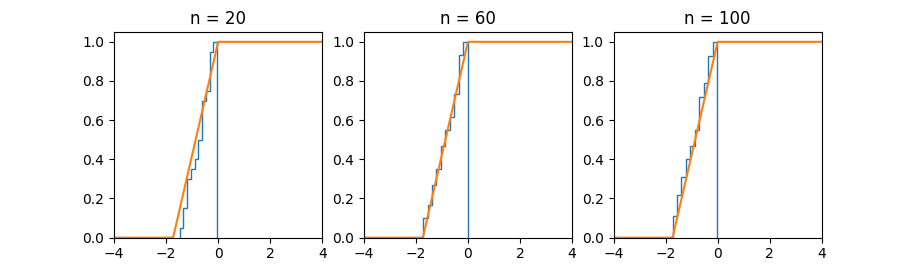
\includegraphics[width=0.8\linewidth]{fig/4norm.png}}
\caption{Нормальное распределение}
\label{fig:box20}
\end{figure}

\begin{figure}[h]
\center{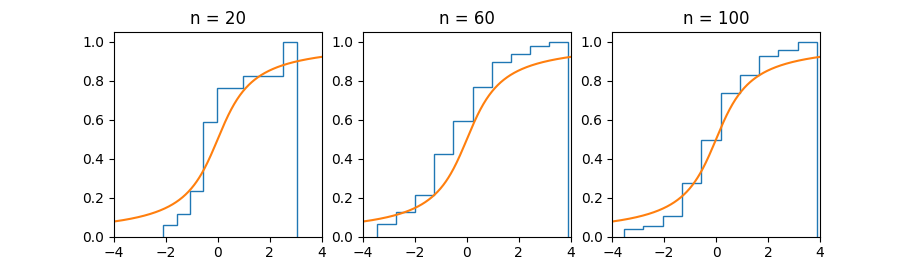
\includegraphics[width=0.8\linewidth]{fig/cauchy4.png}}
\caption{Распределение Коши}
\label{fig:box20}
\end{figure}

\begin{figure}[h]
\center{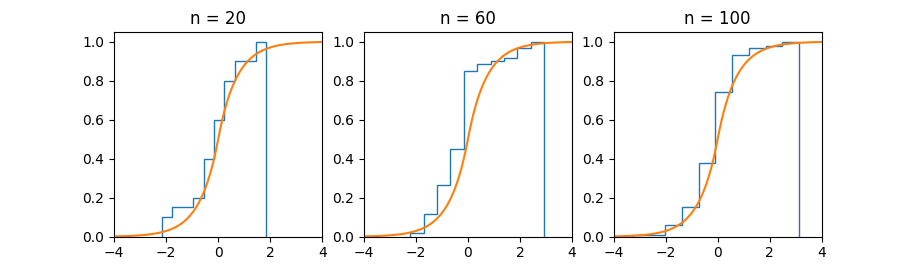
\includegraphics[width=0.8\linewidth]{fig/4laplace.png}}
\caption{Распределение Лапласа}
\label{fig:box20}
\end{figure}

\begin{figure}[h]
\center{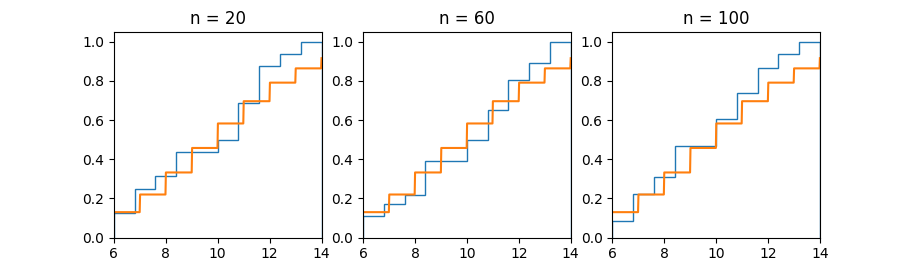
\includegraphics[width=0.8\linewidth]{fig/4poi.png}}
\caption{Распределение Пуассона}
\label{fig:box20}
\end{figure}

\begin{figure}[h]
\center{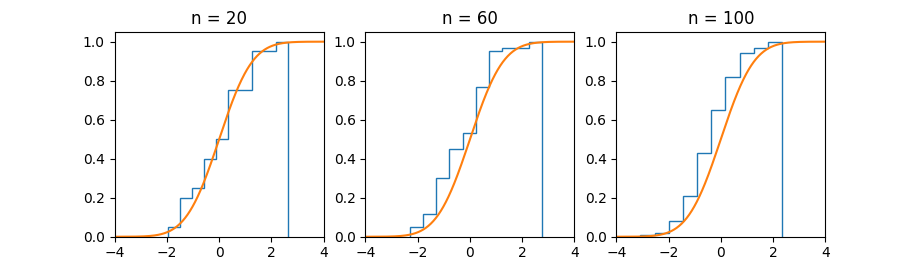
\includegraphics[width=0.8\linewidth]{fig/4uni.png}}
\caption{Равномерное распределение}
\label{fig:box20}
\end{figure}
\section{Обсуждение}
Гипотеза $H_0$ о нормальном законе распределения $N(x, \hat{\mu}, \hat{\sigma})$ при уровне значимости $\alpha = 0.2$ согласуется с выборкой.

\section{Приложение}
Исходный код текста программ можно найти по ссылке \\ https://github.com/mariiabav/MathStatistics.git   

% Не редактируем: Страница библиографии (формируется автоматически из книжек, указанных в refs.bib и пометок \cite{имя_источника} в тексте)
\newpage
\printbibliography[title=Перечень использованных источников]
\addcontentsline{toc}{section}{Перечень использованных источников}
\end{document}
